The home page of our website is shown in \cref{fig:home_page}, the user can access our two main tools through the buttons "solve a graph" and "visualise steps to a solution". In addition we added a section that extended our original scope of our tool, "what is the colourful $k$-center" to introduce the colourful $k$-center problem to users through an example. Although this feature was not part of our original set of requirements, we introduced a step by step example to explain the relationship between the $k$-center and colourful $k$-center, based on the analogies described in \cref{section:k_center}, \cref{section:robust_k_center} and \cref{section:colourful_k_center}. We felt that this served as a gentle introduction to $k$-center problems.

%TC:ignore
\begin{figure}[H]
    \centering
    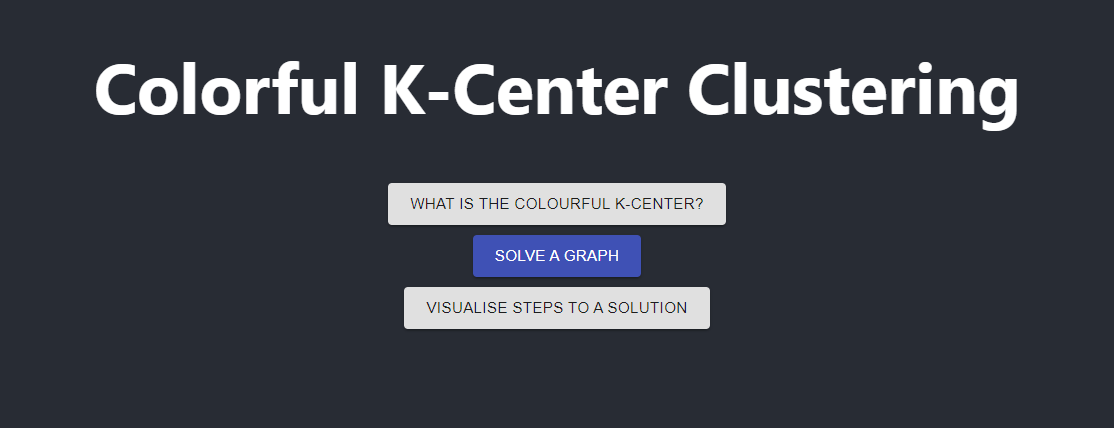
\includegraphics[width=0.75\textwidth]{images/home_page.png}
    \caption{Website home page}
    \label{fig:home_page}
\end{figure}
%TC:endignore

\paragraph{Solution Visualisation}~\\
We created a online tool which implements and visualises all five algorithms described in this paper. Implementing these algorithms served as a good introduction to our understanding of a variety of programming paradigms, including approximation, randomised and memetic algorithms. In addition to fulfilling the primary visualisation requirement, we add quality of life features such as tooltips and an interactive legend (\cref{fig:solve_app}).

%TC:ignore
\begin{figure}[H]
    \centering
    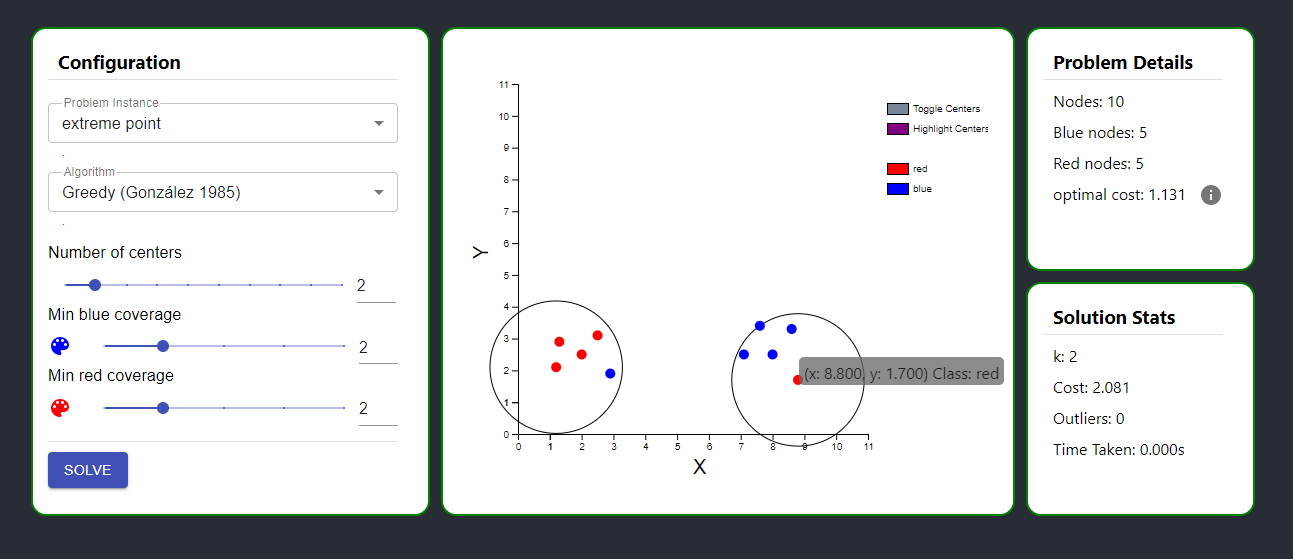
\includegraphics[width=0.85\textwidth]{images/solve_app.png}
    \caption{"solve a graph" web page}
    \label{fig:solve_app}
\end{figure}
%TC:endignore

While tool has the ability to adjust all parameters for the problem instance, there lacks configuration for each individual algorithm. For example, our algorithm implementations have the ability to halt as soon as a target cost or a timeout is reached; this functionality is accessible through the command line but not through the web tool.

\paragraph{Interactive Algorithm Visualisation}~\\
We also provide a tool to show how all five algorithms work step by step. While simpler algorithms such as \emph{Gon} would be understandable to a user without being familiar with the algorithm beforehand, algorithms such as PBS would require prior understanding. If we were reattempt this task, we would add supporting visualisations to show which part of the pseudocode was currently being executed. 

In terms of the genetic algorithm visualisation aspect (see \cref{section:stepped_visualisation}), we believe our design which allows viewing of both the whole population and specific individuals aided our understanding of genetic algorithms. One minor improvement we would make is to highlight specific individuals which were modified between local searches and generations.

A more ambitious extension of our tool would be to add animations to each step to highlight either swaps between centers or opening of new centers. From an educational viewpoint, the effectiveness of this tool remains to be proven. However as far as aiding our own understanding of the algorithms, we believe it has achieved its role.

\paragraph{Accessibility}~\\
Our tool can be accessed at \url{https://colourful-k-center.herokuapp.com}. Considering our project covers algorithms that use LP solvers, this tool provides a way to visualise the O(1)-approximation algorithm without needing to install a solver such as GLPK. Should the user want to run their own instance either locally or on the web, the application is packaged into a Docker image, with build and deploy only requiring two commands (\cref{fig:docker_setup}).

%TC:ignore
\begin{figure}[H]
    \centering
    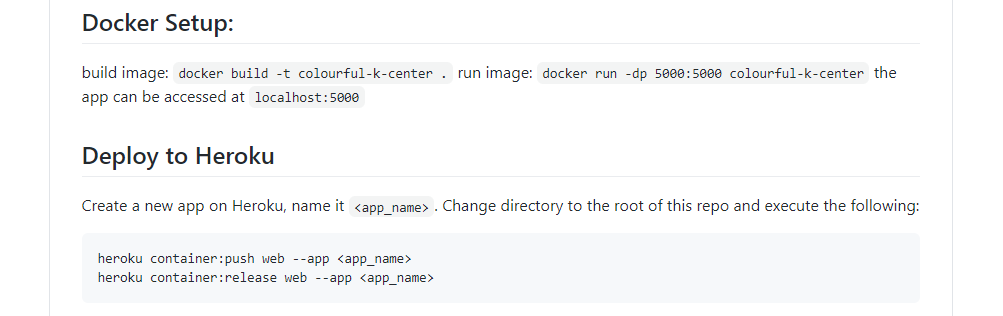
\includegraphics[width=0.85\textwidth]{images/docker_setup.png}
    \caption{Instructions for setting up our web tool using Docker}
    \label{fig:docker_setup}
\end{figure}
%TC:endignore

If a researcher wishes to utilise/extend our code, they would need to install the Python pip dependencies, an LP solver and R (for statistical analysis). Although the latter two dependencies are slightly more involved to install, there are detailed installation guides for both GLPK and R online.